\begin{frame}{$\chi_{b1,2}(1,2,3P) \to \OneS$ fit model}
\begin{columns}
\column{.5\textwidth}
  \centering
  \setlength{\unitlength}{1mm}
  \begin{picture}(50,80)
      %
    \put(0,0){
      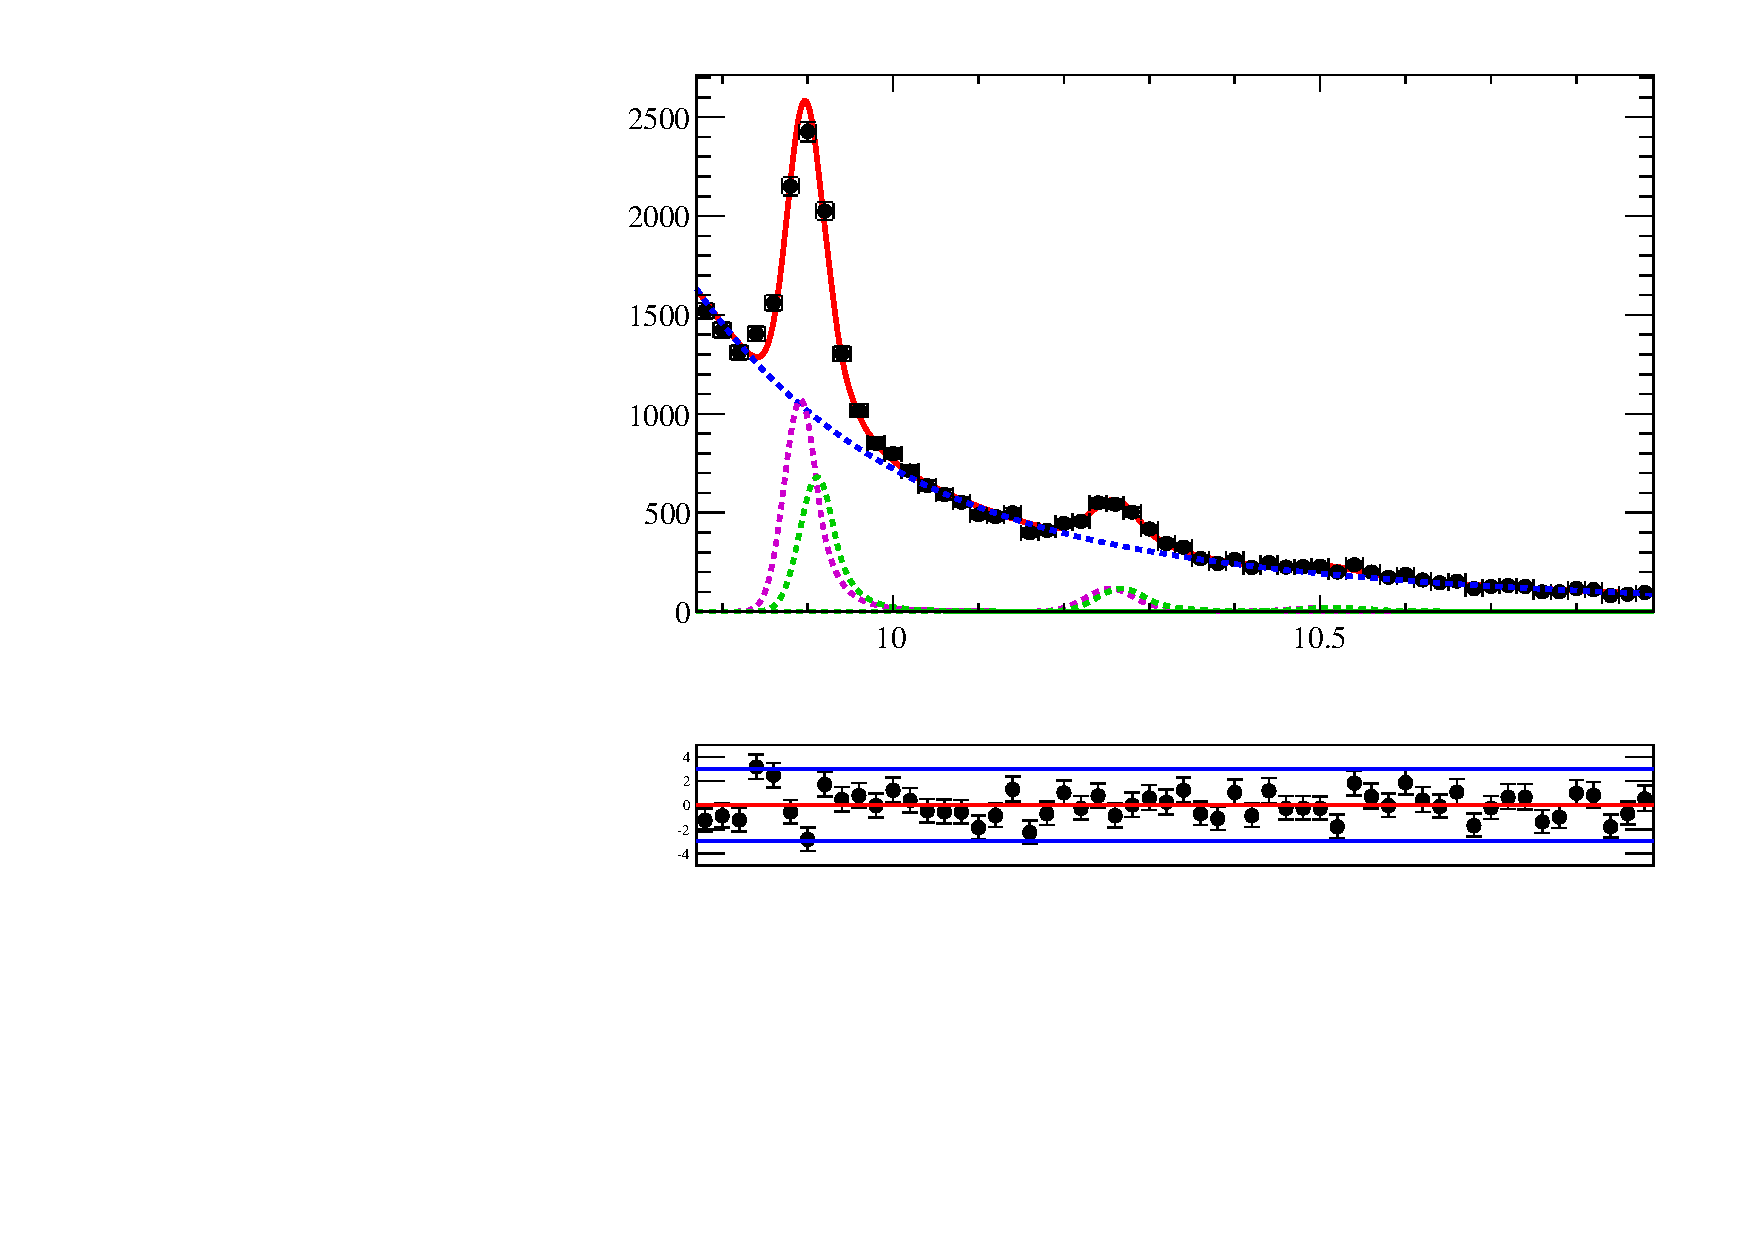
\includegraphics[width=50mm, height=40mm]{chib1s-fit/f2012_fix_14_None}
    }
    
    \put(0,40){
      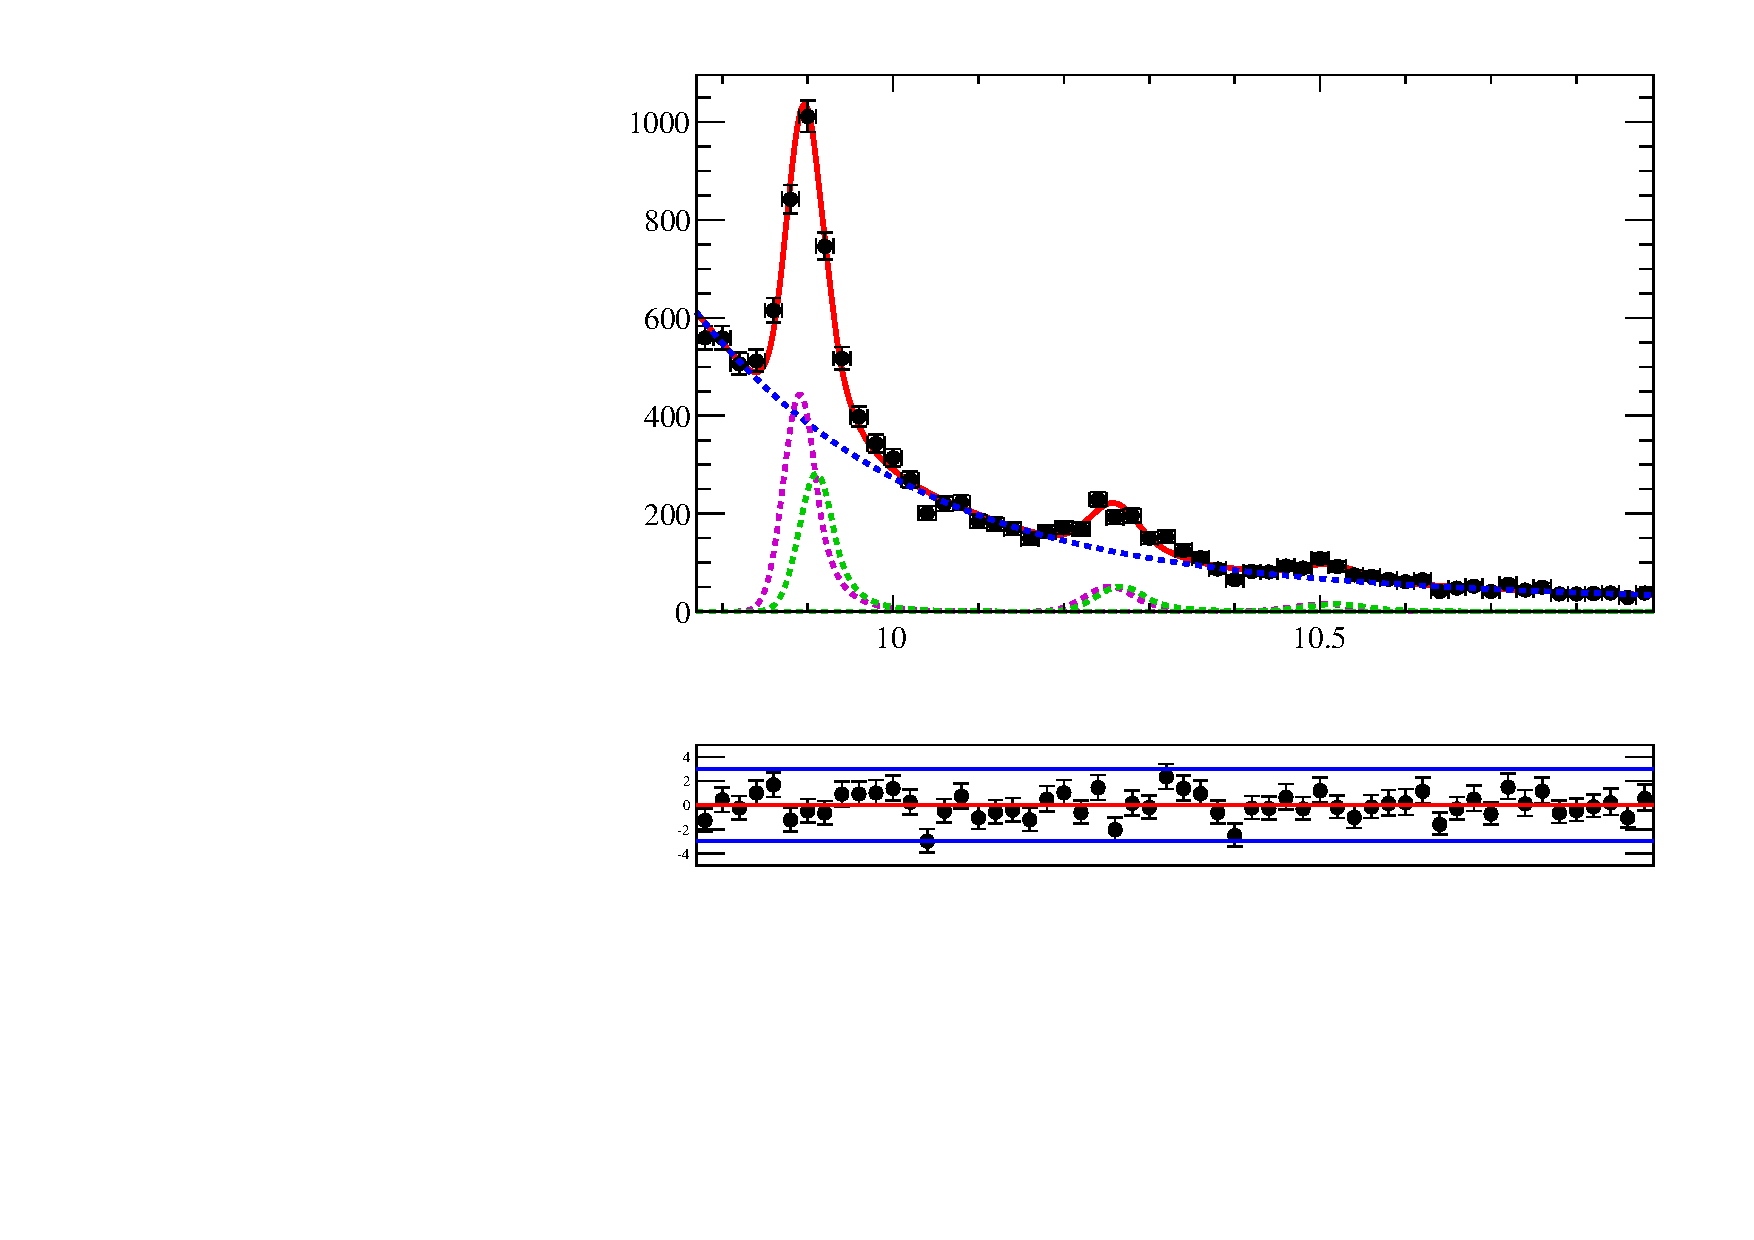
\includegraphics[width=50mm, height=40mm]{chib1s-fit/f2011_fix_14_None}
    }

    \put(0,15){\tiny \begin{sideways}Candidates/(20\mevcc)\end{sideways}}
    \put(5,9.5){\tiny $m_{\mumu \gamma} - m_{\mumu} + 9.4603 \left[\gevcc\right]$}
    \put(25,30){$\sqrt{s} = 8 \tev$}
    \put(20,25){\tiny $p_T(\Y1S) > 14 \gevc$}
    
    \put(0,55){\tiny \begin{sideways}Candidates/(20\mevcc)\end{sideways}}
    \put(5, 49.5){\tiny $m_{\mumu \gamma} - m_{\mumu} + 9.4603 \left[\gevcc\right]$}
    \put(25,70){$\sqrt{s} = 7 \tev$}
    \put(20,65){\tiny $p_T(\Y1S) > 14 \gevc$}
    %\graphpaper[2](0,0)(50, 40)        
  \end{picture}
\column{.5\textwidth}
\begin{itemize}
\item 6 Crystal Ball functions for each of $\chi_{b1,2}(1,2,3P)$ signal (exclude
the study of $\chi_{b0}$ due to its low branching ratio)
\item Product of exponential and linear combination of basic Bernstein
polinomials  for combinatorial background.
\end{itemize}
\end{columns}
\end{frame}
